\documentclass[dvipsnames]{beamer}
\beamertemplatenavigationsymbolsempty
\usecolortheme{beaver}
\setbeamertemplate{blocks}[rounded=true, shadow=true]
\setbeamertemplate{footline}[page number]
%
\usepackage[utf8]{inputenc}
\usepackage[english,russian]{babel}
\usepackage{amssymb,amsfonts,amsmath,mathtext}
\usepackage{subfig}
\usepackage[all]{xy} % xy package for diagrams
\usepackage{array}
\usepackage{multicol}% many columns in slide
\usepackage{hyperref}% urls
\usepackage{hhline}%tables
\usepackage[dvipsnames]{xcolor}

\graphicspath{ {../figures/} }

\begin{document}

\begin{frame}{Anti-Distillation from a simple model to a complex one.}

\textbf{Goal}: Adapting the model to more complex data.

\begin{columns}[c]
\column{0.6\textwidth}
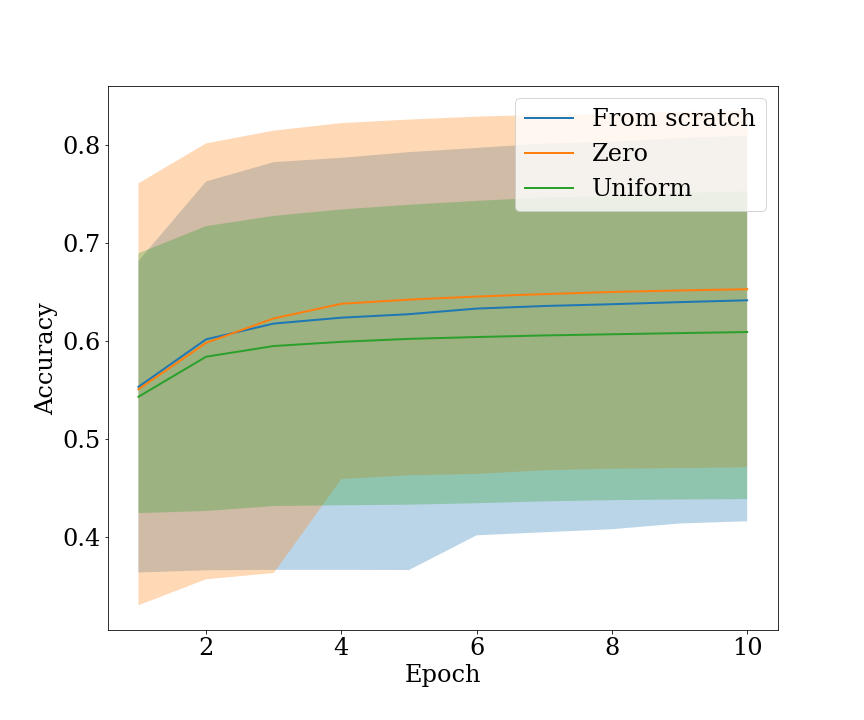
\includegraphics[width=\textwidth]{accuracy.png}
\column{0.5\textwidth}

Increasing complexity:

\begin{enumerate}
    \item More classes
    \item More features
\end{enumerate}

\bigskip

\textbf{Our solution}: Weight initialization using the parameters of the pre-trained model.

\end{columns}

$$\mathbf{w}_1 = \varphi(\mathbf{u}^*)$$
$$\mathbf{w}_1 = (\mathbf{u}^*, \mathbf{w}_1'),\quad \mathbf{w}_1' = {\color{orange}\mathbf{0}}, \quad  \mathbf{w}_1' \sim {\color{OliveGreen} U[-\frac{1}{\sqrt{n}}, \frac{1}{\sqrt{n}}]}$$

\end{frame}

\end{document} 